\documentclass[11pt,a4paper]{report}

\usepackage{url}
\usepackage[utf8]{inputenc}
\usepackage{graphicx}
\usepackage[all]{xy}
\usepackage{adjustbox}
\usepackage[hidelinks]{hyperref}
\usepackage{tikz} 
\usepackage{multirow}
\usepackage{amsmath}
\usepackage{amssymb}
\usepackage{amsthm}
\setlength {\marginparwidth }{2cm}
\usepackage{todonotes}
\usepackage{array}
\usepackage{listings}
\usepackage{longtable}
\usepackage[a4paper]{geometry}
\usepackage[american]{babel}
\usepackage{enumitem}
\usepackage{tabularx}
\usepackage{float}
\usepackage{glossaries}
\usepackage{amssymb}
\usepackage{upgreek}
\usepackage{stmaryrd}
\usepackage{caption}
\usepackage{subcaption}
\usepackage{mathtools}
\usepackage{svg}
\usepackage{dirtytalk}

\makeatletter %otherwise geometry resets everything
\Gm@restore@org
\makeatother

\setlength{\itemsep}{0cm}
\setlength{\voffset}{0cm}
\setlength{\headheight}{0cm}
\setlength{\topmargin}{0cm}
\setlength{\extrarowheight}{3pt} %for superscripts in tabular
\setlength{\arraycolsep}{4pt}
\lstset{basicstyle = \footnotesize, breaklines = true}


\graphicspath{{imgs/}}

\makeglossaries
\loadglsentries{acronyms}

\begin{document}
\begin{titlepage}
\begin{center}
\textsc{\LARGE Research Internship Report\\Software Science}\\[1.5cm]

\includegraphics[height=100pt]{logo}

\vspace{0.4cm}
\textsc{\Large Radboud University}\\[1cm]
\hrule
\vspace{0.4cm}
\textbf{\huge Internship report with some cool name}\\[0.4cm]
\hrule
\vspace{2cm}
\begin{minipage}[t]{0.45\textwidth}
\begin{flushleft} \large
\textit{Author:}\\
Elina Antonova\\
s1057069
\end{flushleft}
\end{minipage}
\begin{minipage}[t]{0.45\textwidth}
\begin{flushright} \large
\textit{Supervisor:}\\
dr. Mairieli Wessel \\
\texttt{mairieli.wessel@ru.nl}\\[1.3cm]
\end{flushright}
\end{minipage}
\vfill
{\large \today}
\end{center}
\end{titlepage}

\begin{abstract}
Very cool abstract to my research
\end{abstract}



\tableofcontents

\chapter{Introduction}\label{introduction}

\glspl{llm} are statistical models that were trained on the large amount of data containing billions of parameters and use previous tokens to predict the future tokens~\cite{gpt-usage-and-lim}. \gls{llm} are used in different domains such as conversation agents, education, text summarisation, explainable AI, information retrieval and many more~\cite{Dale_2021}. One of the most well-known models is \gls{gpt}~\cite{Floridi2020-gpt3paper}, a chatbot developed by OpenAI and first released in November 2022. According to OpenAI CEO Sam Altman, \gls{gpt} reached 100 million weekly active users in November 2023\footnote{https://www.theverge.com/2023/11/6/23948619/openai-chatgpt-devday-developer-conference-news}. 

\gls{gpt} drew so much attention for its detailed and
expressive answers across many domains of knowledge, including software development. The chatbot was adopted by some software engineers as an alternative to using Google for solving software development related issues. Studies have investigated \gls{gpt}'s efficacy when used in software development processes~\cite{Hörnemalm_2023}, its limitations~\cite{gpt-usage-and-lim}, domains of application within issue-tracking systems and reliance on the \gls{gpt}-generated code~\cite{gpt-issue-tracking} and the correctness of the generated code~\cite{gpt-code-correctness, zhang2023critical}. Additionally, some studies focus on the human-bot interaction: the role of
\gls{gpt} in the process of collaborative software architecting~\cite{gpt-software-architecture} or what is \gls{gpt}'s primary use in issue-tracking systems~\cite{gpt-issue-tracking}. 

In this study we focus on the domain of human-bot interaction and use developer prompts to extract the different types of collaboration that developers want \gls{gpt} to follow during their interaction. We expect to see requests for \gls{gpt} to be a pair programmer and work together on issue resolution, where developer provides a feedback on how the chatbot answer can be improved and vice-versa; or it will be asked to review the code and suggest improvements or find a bug in the program. There are many ways developers can collaborate with \gls{gpt} and we focus on extracting some patterns from their prompts to recognise what type of collaboration does developer expect from \gls{gpt}. This leads to the research question of this study: \textbf{What role does \gls{gpt} take in user-chatbot interaction with software developers?}

To answer the research question we use various supervised and unsupervised text mining techniques: n-grams extraction, sequence mining and topic modelling. These methods help us with understanding the common themes and topics present in developers' \gls{gpt} prompts and the expectations they place on \gls{gpt} in these prompts. Sequence mining and topic modelling provide information extracted from the dataset that describes the data, while n-grams is used to provide the initial overview of what are the most common words/word combinations present in the data we are working with. We apply the mentioned techniques on DevGPT~\cite{devgpt} dataset that consists of developer-\gls{gpt} conversations sourced from GitHub\footnote{\url{https://github.com}} commits, pull requests, code files, issues and discussion, and from HackerNews\footnote{\url{https://news.ycombinator.com}}. 

The answer to this research question provides valuable insights into the role that \gls{gpt} plays in developer-chatbot collaboration. Additionally, it shows what tasks developers trust chatbot like \gls{gpt} to perform and what expect from \gls{gpt} in that role. By outlining the collaboration patterns of developer-chatbot interaction, we provide the ground for new research to develop or enhance chatbots' ability to help the software developer in the way that is the most expected from the chatbot.

We firstly provide some background information and related research in Chapter~\ref{related-work}. Then we describe in details what dataset consists of, what pre-processing steps are taken, how the data minins techniques are applied, provide some statistics, outliers and selected methods limitations in Chapter~\ref{methodology}. Chapter~\ref{results} focuses on describing and analysing the results. Chapter~\ref{conclusions} provides an overview of what was done and what results were achieved with this study, and provides the discussion of the project and possible future research. 

\chapter{Background}
\section{ChatGPT and interaction with it}
\gls{gpt} is a large-scale, pre-trained language model developed by OpenAI and designed to engage in natural language conversations, utilising \gls{nlp} techniques that enable generation of the human-like text with context and coherence. Its performance in generating creative and novel text and ability to adapt to the context opened the possibilities for applications in various fields, such as creative writing, marketing, advertising, technical problem solving, etc~\cite{fi15060192}. 

\gls{gpt} model is a transformer-based neural network~\cite{vaswani2017attention} crafted to accomplish natural language processing tasks. Initially the prototype was launched on 30 November 2022, which became available to public on 30 January 2023. The model is trained on vast corpus of textual data that was gathered from various sources, such as articles, books, reviews, online conversations and other human-generated data. This allowed model to capture natural language patterns, nuances, complexities allowing \gls{gpt} to perform well in non-trivial dialogues on various topics. 

This research focuses on the interactions with \gls{gpt}. Interaction with \gls{gpt} consists of \textit{conversation}, which is a collection of pairs of user \textit{prompt} and \gls{gpt}'s reply. The comversation starts with user creating the initial \textit{prompt} which usually consists of the problem description, question, background information, step-by-step instruction for \gls{gpt} or any other information relevant to the user needs. \gls{gpt} uses the information provided in the prompt to generate the \textit{response}. After user receives the response they can either stop the conversation or continue it with providing the new prompt for \gls{gpt} to process. Such \gls{gpt} conversations are used in this reseatch to answer the posed research questions with extensive user prompt analysis.

\section{Related works} \label{related-work}
DevGPT~\cite{devgpt} is a well-researched dataset that provides various insights into the developer-ChatGPT interactions and the usability of ChatGPT in the field related to software engineering. 

The DevGPT dataset provides great opportunities to evaluate how ChatGPT handles questions and requests related to code generation and debugging, and how well the generated code corresponds to the set standards of code security, cleanliness, and efficiency. Several studies analyzed various aspects of the generated code: some studies focused on the security aspect and many other studies on the quality aspect of the generated code. The studies done by Siddiq, et al.~\cite{siddiq2023generate} and Rabbi, et al.~\cite{gpt-code-security-quality} revealed that the generated and modified code contained several CWE (Common Weakness Enumeration)\footnote{\url{https://cwe.mitre.org}} vulnerabilities, and issues captured by the Pylint 3.0.2\footnote{\url{https://pypi.org/project/pylint/3.0.2/}} code quality analysis tool. Moreover, Zhang, et al.~\cite{zhang2024-code-smell} showed that at least 35\% of the 98 generated Kubernetes manifests contained at least one instance of a code smell. Other studies that researched the generated Python and Java code have discovered various code safety and quality issues by analyzing the generated code~\cite{clark2024-quantitative-quality-analysis,Moratis2024-code-quality,Siddiq2024-code-quality}. Moratis et al.~\cite{Moratis2024-code-quality} and Siddiq et al.~\cite{Siddiq2024-code-quality} investigated the direct use of generated code in the source code base and concluded that ChatGPT generated code has to be reviewed and often modified if it is to comply with the code safety and quality standards. 

Researchers are also exploring the structure, topics, and outcomes of interactions between developers and ChatGPT. Several studies using the DevGPT dataset have focused on analyzing the developers' intent and the subjects of their requests. Study conducted by Sagdic, et al.~\cite{sagdic2024-devgpt-taxonomy} have used BERTopic~\cite{grootendorst2022bertopicneuraltopicmodeling} topic modelling \acrshort{nlp} technique to create topic clusters, which can be manually labeled and added to the topic's taxonomy. They have discovered seventeen topics that can be placed in seven categories: advanced programming; front- and backend development; DevOps integration and practices; streaming, media and localization; data management; and other topics. Similar approach was used by Mohamed, et al.~\cite{Mohamed2024-topics}, where they have used four different classifiers to categorize all conversations by their purposes based on the developer needs. Their research revealed 19 categories, out of which code generation and seeking general information accounted for almost third (31.15\%) of all the conversations. Champa, et al.~\cite{champa2024-gpt-use} have used \textit{facebook/bart-large-mnli} model for zero-shot classification~\cite{lewis2019bartdenoisingsequencetosequencepretraining} to categorize the types of tasks developers present to ChatGPT, where they discovered that quality management of Python code and commit issue resolution tasks were the categories developers seeked the most assistance with. While all three studies share a common goal of categorizing developer interactions with ChatGPT, they differ in methodology and focus --- ranging from topic modeling to classification based on intent --- yet consistently highlight code generation and problem-solving as dominant use cases.

Recent studies have analyzed various aspects of integrating ChatGPT into multi-language software development and pull request workflows. Aguiar, et al.~\cite{aguiar-multilang-chatgpt} found that over 75\% of ChatGPT's code suggestions used a different language than the host repository, with the highest mismatch in CSS (91.16\%) and the lowest in C\# (60.18\%) and CodeQL (58.08\%). Chouchen, et al.~\cite{chouchen2024-pr-how} examined the topics of ChatGPT-related pull request conversations, identifying common themes such as code generation, refactoring, bug fixing, concept explanation, DevOps, testing, and recommendations, and noted that ChatGPT was more frequently used in large, time-consuming pull requests. Watanabe, et al.~\cite{watanabe-code-review-chatgpt} and Hao, et al.~\cite{Hao2024-pr-exporatory} found that developers generally responded positively to ChatGPT's code review comments, with fewer than one-third of replies expressing disagreement. Additionally, Hao, et al.~~\cite{Hao2024-pr-empirical} observed that ChatGPT was used across various roles in GitHub pull requests and issues, including as an author, reviewer, and collaborator. Together, these studies highlight ChatGPT’s growing presence and generally positive reception in collaborative software development environments. However, the responses should be critically checked as they still tend to contain code snippets written in non-native language. 

Several recent studies have analyzed ChatGPT's effectiveness in addressing code generation and code refactoring tasks. Grewal, et al.~\cite{Grewal2024-codegen} and Jin, et al.~\cite{Jin2024-codegen} investigated its use for code generation, concluding that while ChatGPT can produce functional code, developers often need to verify its correctness and adjust the structure to meet the functional requirements. Code refactoring, on the other hand, is a more open-ended task, where ChatGPT tends to focus on improving readability, maintainability, usability, and performance, as shown by Chavan, et al.~\cite{Chavan2024-refactoring} and AlOmar, et al.~\cite{AlOmar2024-refactoring}. Their research revealed that developers typically adopt a straightforward strategy --- copying the code and directly requesting a refactor --- which resolves the issue in an average of 2.7 to 4.6 prompts. Prompt quality is also a critical factor in successful interactions with ChatGPT~\cite{Mondal2024-prompts-issues, Wu2024-promptpatterns}. Mondal, et al.~\cite{Mondal2024-prompts-issues} found that vague or underspecified prompts, especially those requesting additional features without clear specifications, often lead to longer and less efficient conversations. Altogether, these studies suggest that while ChatGPT is a valuable tool for code-related tasks, its effectiveness heavily depends on prompt clarity and developer oversight.
\chapter{Data}\label{sec:data}
To answer the research question, we used the DevGPT dataset~\cite{devgpt}, which contains \acrshort{gpt} conversations shared on GitHub and Hacker News between late May 2023 and October 12, 2023. The dataset includes nine snapshots (latest: October 12, 2023), each comprising links to \acrshort{gpt} conversations found in GitHub commits, issues, discussions, pull requests, code files, and Hacker News articles.

In this study, we use data from all available snapshots. To ensure data quality, we removed duplicate entries based on shared \acrshort{gpt} conversation links. Additionally, we extended the DevGPT dataset with a new dataset collected in March 2025. This extension contains developer-chatbot conversations shared in the same sources but posted after the latest DevGPT snapshot. The structure of the extended dataset mirrors that of DevGPT to maintain consistency.

Table~\ref{table:data_stat} presents the number of unique conversations in each dataset and in total, along with the remaining number of conversations after removing duplicates and non-English conversations.

\begin{table}[h]
    \centering
    \resizebox{\textwidth}{!}{%
    \begin{tabular}{|l|c|c|c|c|c|c|c||c|}
        \hline
        & Commits & Issues & Discussions & Pull req. & Code files & Repositories & Hacker News & Total \\
        \hline
        DevGPT DR & 670 & 516 & 59 & 268 & 2010 & 0 & 322 & 3845\\
        \hline
        Extension DR & 881 & 1134 & 65 & 775 & 9536 & 10 & 805 & 13206 \\
        \hline
        Combined DR & 896 & 1235 & 113 & 813 & 9959 & 10 & 858 & 13884 \\
        \hline
        Combined NE & 858 & 986 & 89 & 665 & 7968 & 8 & 755 & 11329 \\
        \hline
    \end{tabular}
    }
    \caption{Number of conversations after all the duplicates (DR) and non-English conversations (NE) were removed from the data.}
    \label{table:data_stat}
\end{table}

The total number of conversations shared across all the sources is 13884. However, after removing duplicate conversations from the entire combined dataset, it leaves us with 12574 conversations, which means that 1310 \linebreak developer-\acrshort{gpt} conversations are shared in multiple locations. However, dataset contains only 10146 unique conversations out of 11329 conversations sourced from all seven locations after non-english conversations are removed.

\section{Data cleaning}
During our initial analysis of the dataset, we identified the presence of information irrelevant to the research question --- referred to as ``noise''. First, many prompts contain embedded code alongside natural language. Second, while we focus exclusively on English-language conversations, the dataset includes interactions in multiple languages. Both factors introduce noise that must be removed before proceeding with data exploration and answering the research questions.

\subsection{Code detection and its accuracy}\label{sec:prog-identification}
Initially we attempted to detect programming language content using the Guesslang Python library\footnote{\url{https://pypi.org/project/guesslang/}}, but its accuracy and recall were too low for our dataset. As a result, we developed a custom method for identifying and filtering out programming lines.

To identify code segments within prompts, we first split each prompt into individual lines using the line break character (\textit{\textbackslash n}). We then applied a custom script to estimate the likelihood that each line contains code. This approach is based on the assumption that code blocks typically appear on separate lines from natural language text and often span multiple lines within a prompt. As a result, line-by-line analysis is necessary to accurately detect code.

To identify whether a line is written in a programming language or natural language, we implemented a function that evaluates the line’s structures --- whether they are tokens or full sentences --- and assigns them a probability score: \texttt{0} indicates a programming language structure, \texttt{0.5} indicates ambiguity (could be either), and \texttt{1} indicates natural language. The list below shows what kind of structures are considered in this script:
\begin{itemize}
    \item Line is empty (likelihood: 0);
    \item Line starts a multiline comment block with symbols like \texttt{/*}, \texttt{"""}, \texttt{'''}, or \texttt{<!--}, and does not end on the same line --- the whole block is marked as comment (likelihood: 0);
    \item Line is within a multiline comment block and ends with symbols like \texttt{*/}, \texttt{"""}, \texttt{'''}, or \texttt{-->} --- marked as comment (likelihood: 0);
    \item Line matches single-line comment patterns such as \texttt{//}, \texttt{\#}, \texttt{--}, etc. --- marked as comment (likelihood: 0);
    \item Line starts with an opening HTML tag (e.g. \texttt{<div>}) and does not end with a closing tag --- line and subsequent lines until closing tag are marked as HTML (likelihood: 0);
    \item Line contains a complete HTML block (e.g. \texttt{<p>Text</p>}) --- marked as HTML (likelihood: 0);
    \item Line is tokenized using \texttt{shlex.split} if it contains quotes, otherwise by whitespace. Each token (word) is assigned a probability score based on specific heuristics:
    \begin{itemize}
        \item Word contains space and resembles a sentence --- averaged likelihood from subword analysis;
        \item Word starts with tab (likelihood: 0);
        \item Word is in a list of known programming keywords (likelihood: 0.5);
        \item Word is a camelCase or PascalCase identifier (likelihood: 0);
        \item Word is in UPPERCASE (e.g. SQL keywords; likelihood: 0.5);
        \item Word is purely alphabetical (likelihood: 1);
        \item Word is a comment-like or inline programming pattern (e.g. \texttt{::}, \texttt{\#}, \texttt{<\textbackslash }, \texttt{<|-};  likelihood: 0);
        \item Word matches function calls, method chains, array indexing, or regular programming syntax (e.g. \texttt{func(x)}, \texttt{obj.attr}, \texttt{arr[i]}; likelihood: 0);
        \item Word ends with punctuation (e.g. \texttt{word,}, \texttt{word.}, \texttt{word:}; likelihood: 0.5);
        \item Word ends with semicolon often used in programming syntax (likelihood: 0);
        \item Word lacks alphabetic characters (likelihood: 0);
        \item All other cases (likelihood: 1).
    \end{itemize}
\end{itemize}

To determine whether a line is written in natural language or code, the script calculates the average likelihood score by summing the individual scores of all structures (tokens or sentences) in the line and dividing by the total number of structures. If the resulting average is above 0.5, the line is considered to contain natural language; otherwise, it is classified as a code line.

The effectiveness of the code detection script was evaluated using ten randomly selected conversations, from which up to 20 lines were randomly sampled. These lines were processed by the script, and the results were saved to a file. Each line was then manually labeled as either code or non-code for comparison. The script demonstrated satisfactory performance across all tested conversation sources. Table~\ref{table:script-accuracy} shows how well the code detection script works.

\begin{table}[h]
    \centering
    \begin{tabular}{|l|c|c|}
        \hline
        & Accuracy & F-score  \\
        \hline
        GitHub commits & 0.96 & 0.98 \\
        \hline
        GitHub issues & 0.92 & 0.95 \\
        \hline
        GitHub discussions & 0.92 & 0.93 \\
        \hline
        GitHub pull requests & 0.96 & 0.97  \\
        \hline
        GitHub code files & 0.95 & 0.96  \\
        \hline
        GitHub repositories & 0.91 & 0.94  \\
        \hline
        Hacker News & 0.92 & 0.94  \\
        \hline
        \textbf{Total} & \textbf{0.92} & \textbf{0.95}  \\
        \hline
    \end{tabular}
    \caption{Accuracy and F-score of the code detection script per data source category.}
    \label{table:script-accuracy}
\end{table}

False-positives and false-negatives were examined to better understand the types of errors made by the code detection script. The most common false-negatives occurred with error messages or log outputs, which often contain large amounts of natural language, making them difficult to distinguish from regular text. On the contrary, sentences with a high number of punctuation marks were frequently misclassified as code, even when they were not. For instance, lines such as \textit{``Done.''} and \textit{``- Prefer async/await over promises!''} were incorrectly identified as code, although they could plausibly be part of natural language text.

This evaluation method also has limitations, particularly in handling multi-line HTML or comment blocks. Because lines for testing are selected randomly, it is possible to include a line that starts a multi-line HTML tag or comment block without capturing the corresponding closing line. As a result, following lines may be incorrectly labelled as part of HTML or a comment.

Despite these limitations, the script achieved an average accuracy and F-score of over 90\%, which we consider a good result for the purposes of this research.

\subsection{Language detection}
For language detection, we used two existing libraries: \textit{langdetect\footnote{\url{https://pypi.org/project/langdetect/}}} and \textit{pycld2 (Compact Langauge Detect 2)\footnote{\url{https://pypi.org/project/pycld2/}}}. Using both libraries improves detection accuracy --- if one library fails to identify the language, the result from the other helps determine whether the prompt should be kept (if detected as English) or discarded.

The language identification process operates at the line level: each prompt is split into individual lines, and the language is identified for each line separately. If a line is detected as containing only programming code (as described in Section~\ref{sec:prog-identification}), it is marked as code and excluded from language detection. This approach helps avoid misclassifying non-English prompts as English due to the presence of English keywords commonly found in code.

The output of the language check is a tuple, where the first element represents the result from \textit{langdetect}, and the second from \textit{pycld2}. If the most common tuple across all lines in the prompt is either \textit{(``en'', ``en'')}, \textit{(``en'', ``un'')}, or \textit{(``un'', ``en'')}, the prompt is considered to be in English. Any other combination results in the prompt being discarded.


\section{Data exploration}
As part of the data exploration process, we begin by extracting key information about the dataset. Before presenting the statistical overview, it is important to clarify the terminology used in this section. In interactions with \acrshort{gpt}, users submit inputs referred to as \textit{prompts}, which the model uses to generate responses. A sequence of such prompt–response pairs within the same discussion thread creates a \textit{conversation}. For the purposes of this study, we focus exclusively on the user-generated prompts and disregard the responses produced by \acrshort{gpt} across all conversations.

\subsection{Statistics and outliers}
This section covers some statistics regarding the length of the conversations and prompts and the outliers encountered during data exploration process. 

\subsubsection{Number of prompts in conversations}
To better understand the structure and variability of the dataset, we examine the distribution of conversation lengths across different data sources. Table~\ref{table:conv-lengths} shows the basic statistics of conversation lengths across different data sources. Most datasets contain short conversations on average, with median lengths between 1 and 2 prompts, suggesting that interactions are typically brief. However, GitHub repositories stand out with a higher mean (21.38) and median (10.5), as well as the largest standard deviation (31.58), indicating a wider spread and the presence of longer discussions. This phenomenon can be explained by a low number of sharings (8 after non-English conversations removal), where each heavily influences the data.

\begin{table}[H]
\centering
\begin{tabular}{l||c|c|c}
Source           & Mean & Median & Standard deviation \\ \hline
GH Commits       & 3.2   & 1     & 5.65               \\
\hline
GH Issues        & 4.57  & 2     & 8.9                \\
\hline
GH Discussions   & 4.66  & 2     & 9.52               \\
\hline
GH Pull requests & 3.36  & 2     & 7.94               \\
\hline
GH code files    & 6.72  & 2     & 16.74              \\
\hline
GH repositories  & 21.38 & 10.5  & 31.58              \\
\hline
HackerNews       & 4     & 1     & 9.12             
\end{tabular}   
\caption{Median, mean and standard deviation of the conversation lengths from different sources.}
\label{table:conv-lengths} 
\end{table}

Figure~\ref{fig:conv-per-prompt} contains histograms that show how many conversations contain certain number of prompts, where the conversations with the maximum number of 30 prompts are shown. All the conversations that exceeded the number of 30 prompts were separated in the separate JSON files and their content was investigated and described below. 

\begin{figure}[H]
    \centering
    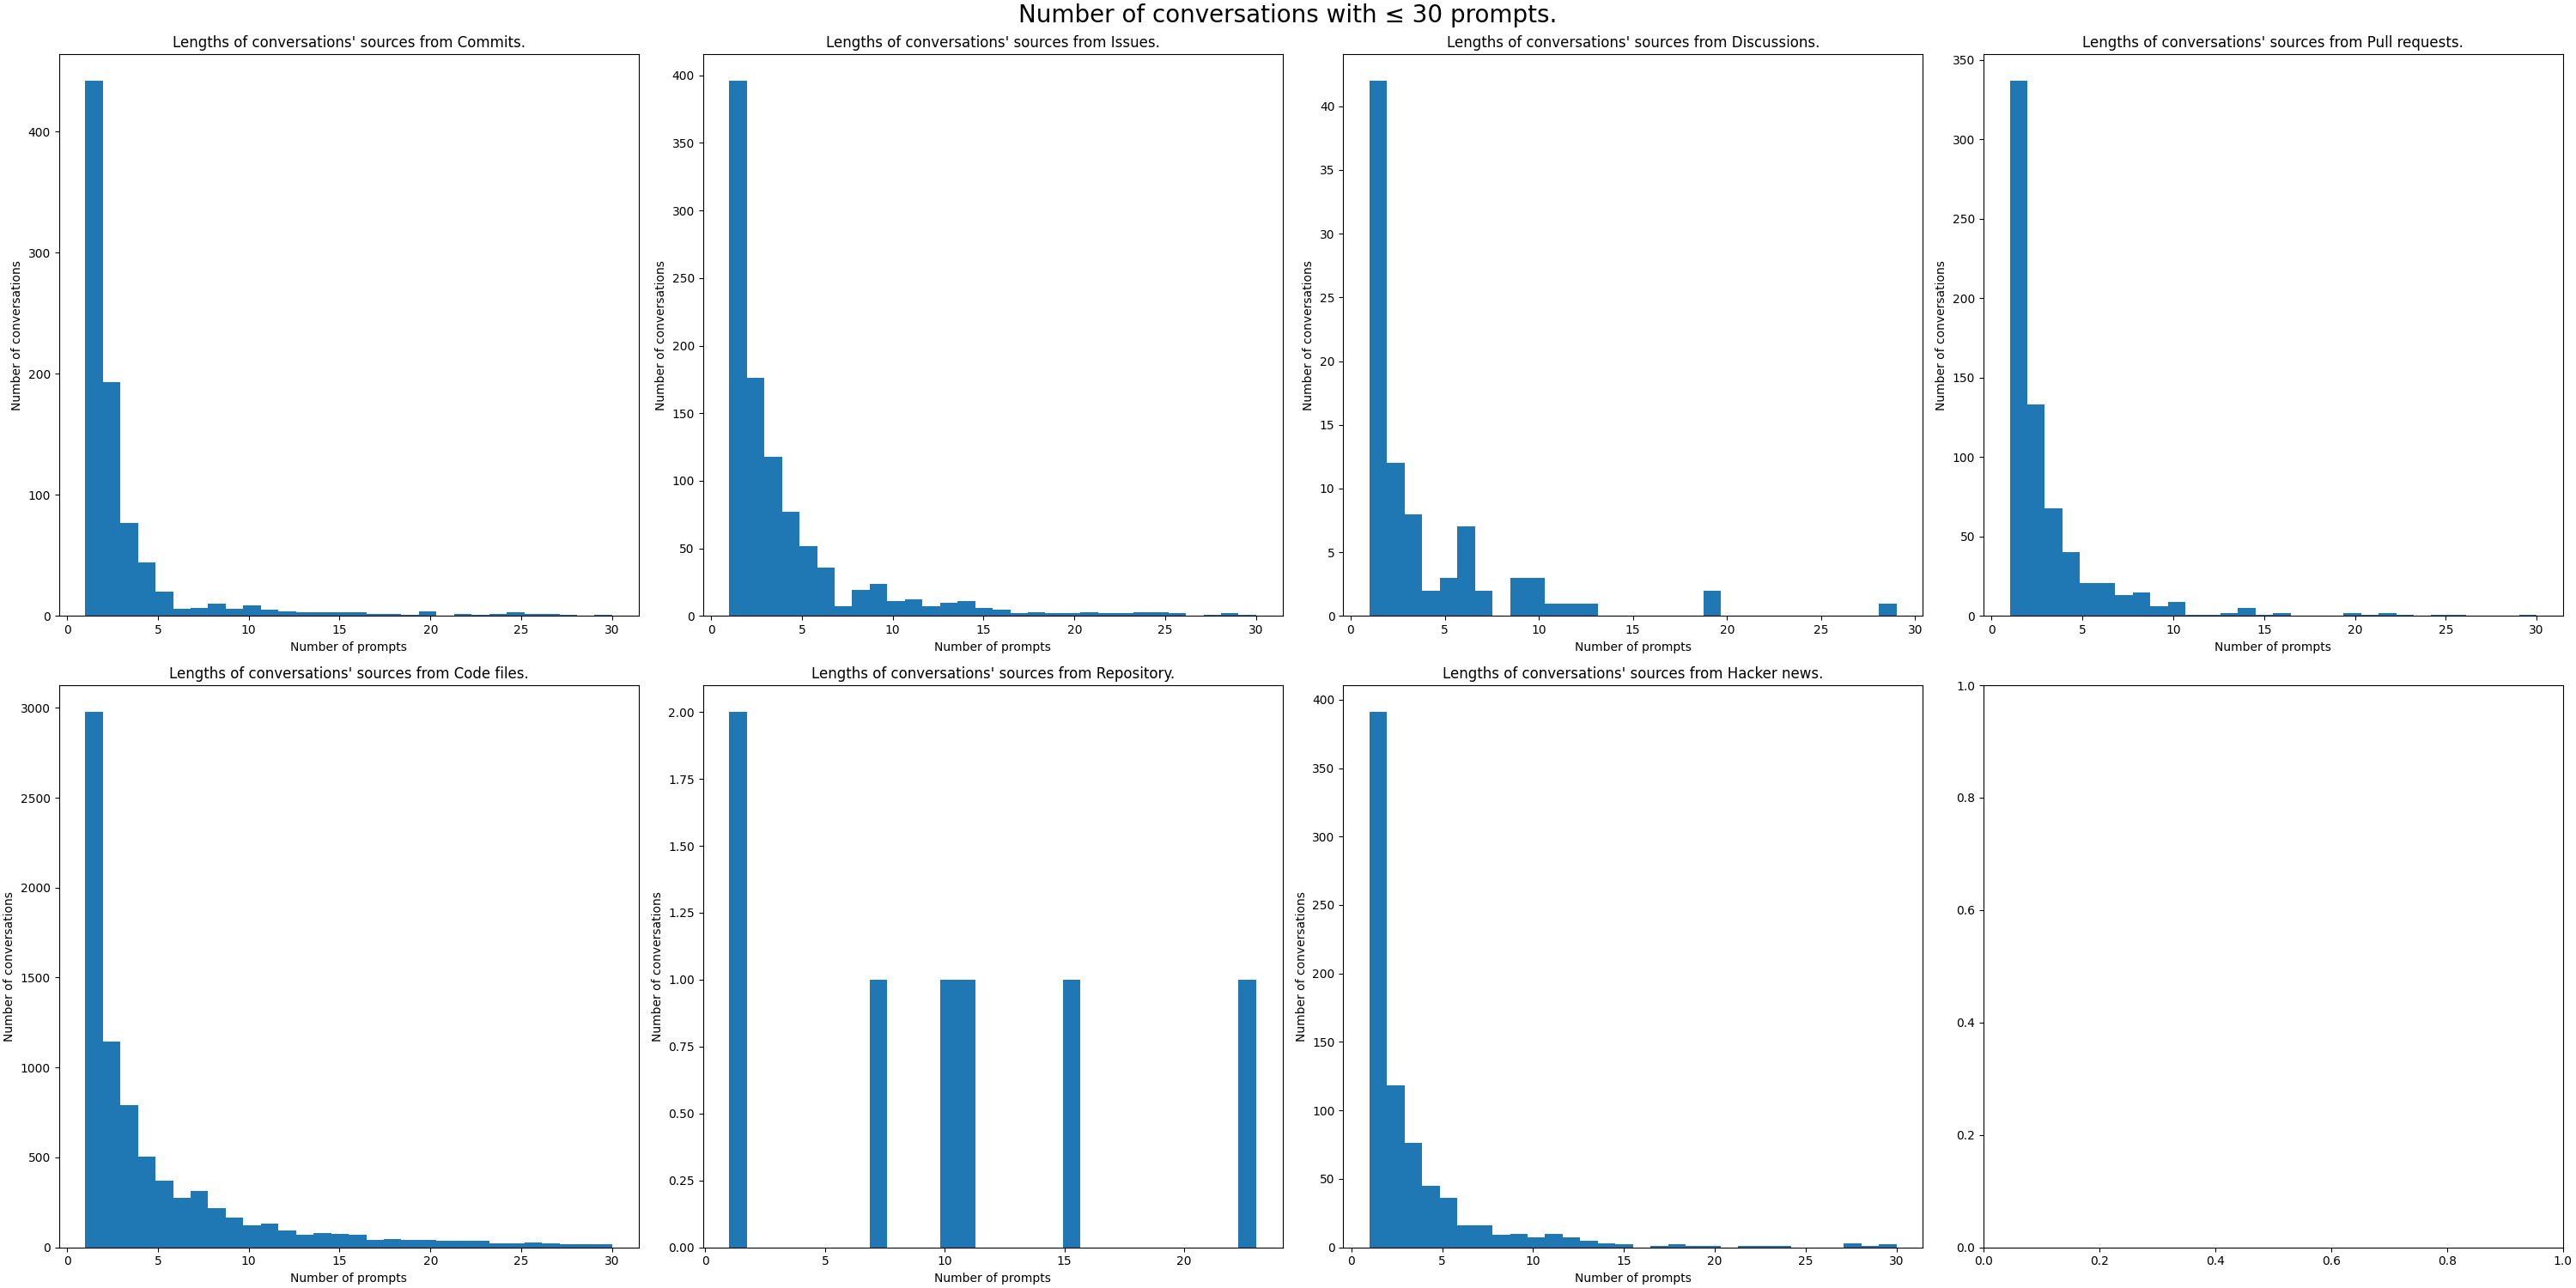
\includegraphics[width=\textwidth]{imgs/conv-per-prompt-nr.png}
    \caption{Lengths of conversations in histogram gathered from different sources.}
    \label{fig:conv-per-prompt}
\end{figure}

\subsubsection{Long conversations contents}
To understand the reasons behind unusually long conversations, we manually reviewed conversations that exceeded a predefined length threshold. The most common patterns are summarised below:

\begin{itemize}
    \item \textbf{Pasted content:} Users split large texts (e.g., code files, articles, books) into multiple prompts due to the prompt's character limits.
    \item \textbf{Iterative debugging:} Users refined requests or sought help with errors after initial code responses did not meet their expectations.
    \item \textbf{Programming assistance:} Users guided \acrshort{gpt} through multi-step coding tasks, testing and iterating on output.
    \item \textbf{Mentorship:} Users shared their own code for feedback, explanations, or improvement suggestions.
    \item \textbf{General discussion:} Some conversations focused on non-programming topics such as advice, opinions, or general discussions.
\end{itemize}

\subsubsection{Average symbol/word count per prompt}
The average number of symbols per prompt varied across sources, as shown in Figure~\ref{fig:symbols-per-prompt}. The \textit{x}-axis represents the prompt position within a conversation, while the \textit{y}-axis shows the average symbol count for that position. Since longer conversations are less common, later prompt positions often reflect fewer data points --- leading to the prompt average pattern changes that can be visibly observed in the conversations sourced from GitHub code files or Hacker News. Across majority of the sources, initial prompts typically have higher symbol counts, as they often introduce the problem in detail.

\begin{figure}[H]
    \centering
    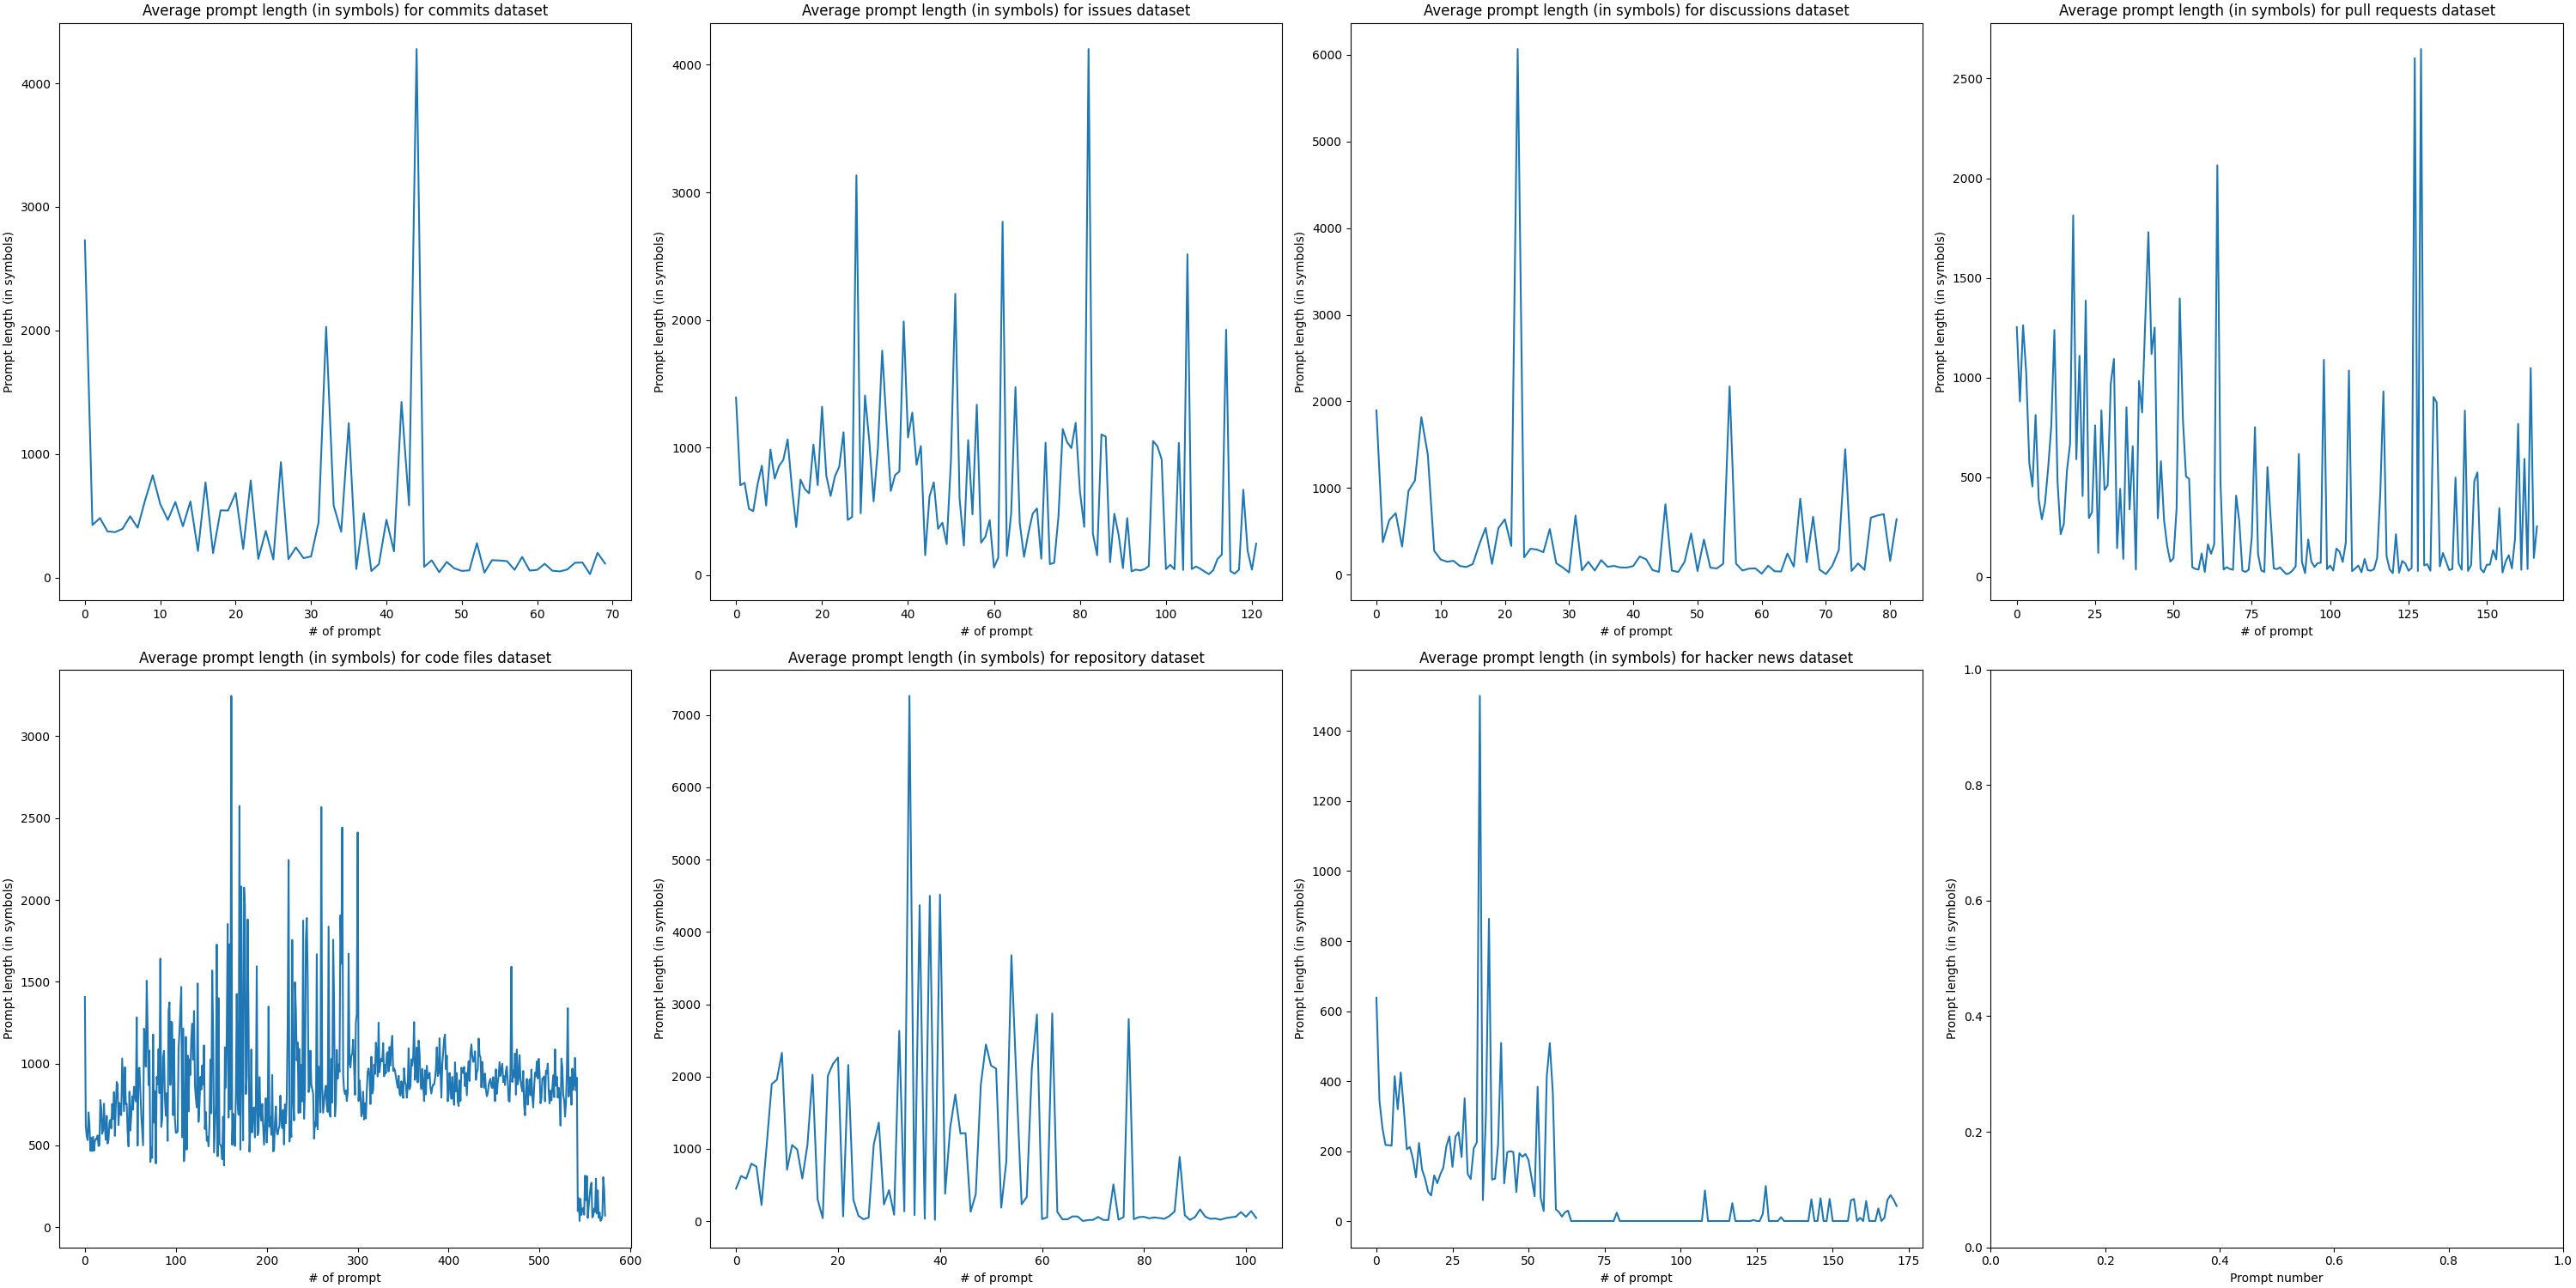
\includegraphics[width=\textwidth]{imgs/symbols-per-prompt.png}
    \caption{Average symbol count per prompt number for all conversation sources after code lines were removed.}
    \label{fig:symbols-per-prompt}
\end{figure}

To identify outliers, we defined dataset-specific cut-off thresholds set at two-thirds of the maximum observed average. Conversations containing prompts exceeding these thresholds were saved for further analysis.

\subsubsection{Long prompt contents}
Conversations containing unusually long prompts were saved and manually reviewed to understand their content. We identified several common reasons for the prompt length:
\begin{itemize}
    \item \textbf{Pasted external content:} Users copied large texts from sources such as scientific articles, GitHub issues, or documentation, often asking for summaries, explanations, or audience-specific rewrites.
    \item \textbf{Code-related debugging:} Prompts included error messages, undocumented code, or comments not flagged as code, with users seeking help with debugging or improvement.
    \item \textbf{Detailed problem descriptions: } Some users provided extensive background to frame their query, including:
    \begin{itemize}
        \item Highly specific requests or detailed issue descriptions;
        \item Roleplay-style prompts (e.g., asking \gls{gpt} to act as a mentor or expert);
        \item Contextual or background information;
        \item Multiple follow-up questions or clarifications;
        \item Previously attempted (but unsuccessful) solutions;
        \item Long URLs or resource links;
        \item Lists of requirements or instructions;
        \item Desired output examples or target functionality.
    \end{itemize}
\end{itemize}

\chapter{Methodology} \label{methodology}
The purpose of investigating how developers use \gls{gpt} for their projects is to gain the necessary knowledge of the roles chatbot plays in developer-bot collaboration in order to enhance its ability to help developers with their requests. In order to extract the knowledge we firstly cleaned the data, investigated what it consists of and applied topic modelling and sequence mining in order to extract the patterns from developer-chatbot collaboration. 

\section{Data} \todo{discuss that DevGPT dataset was extended with more data}
To answer the research question we have used DevGPT dataset~\cite{devgpt}, which consists of the \gls{gpt} conversations that were shared on GitHub and Hacker News between late May 2023 and the 12th of October 2023. The dataset consists of 9 snapshots (latest: 12th of October, 2023), and each snapshot contains the links collected from GitHub commits, issues, discussion, pull requests, code files, and Hacker News (HN) articles. In this research we use the data from all of the available snapshots. However, to keep the data clean, we remove all the duplicate data based on the shared \gls{gpt} conversation links. Table~\ref{table:data_stat} shows the number of conversations that is left after all the duplicates were removed from the dataset (\textit{DR} row).

\begin{table}[h]
    \centering
    \begin{tabular}{|l|l|l|l|l|l|l|}
         \hline
        & Commits & Issues & Discussions & Pull req. & Code files  & HN  \\
         \hline
        DR & 670 & 516 & 59 & 268 & 2010 & 322\\
         \hline
        NE & 659 & 433 & 51 & 227 & 1616 & 290\\
        \hline
    \end{tabular}
    \caption{Number of conversations after all the duplicates (DR) and non-English conversations (NE) were removed from the data.}
    \label{table:data_stat}
\end{table}

\section{Data cleaning}
At the initial investigation of the data, we discovered that the data contains some information that is not needed to answer the research question of this paper (further referred to as "noise"). Firstly, we only focus on conversations in English, while the dataset contains other languages used for communication with \gls{gpt}. Secondly, in addition to natural language, the prompts  contain program code as a part of the prompt text. Both these factors make the data noisy and require to be dealt with before the data exploration and RQ answering is done. 

\subsection{Language detection}
For the language detection purposes we have used existing libraries: \textit{langdetect\footnote{\url{https://pypi.org/project/langdetect/}}} and \textit{pycld2 (Compact Langauge Detect 2)\footnote{\url{https://pypi.org/project/pycld2/}}}. These two libraries are used to ensure higher accuracy at language detection: if one of the libraries is unable to detect the language, then the other library results influence the decision whether to keep the prompt (if it is detected as English text) or discard. 

For language identification process the prompt is divided into lines and the language is identified for each line. If the line consists of the programming code only, then the line is marked as program (details in Section~\ref{sec:prog-identification}) and the language identification is skipped for this line. This is done in order to avoid prompts in non-English language containing a lot of code lines, which have a lot of English words/keywords, to be identified as an English prompts. The result or language check is a tuple, where the first value is the language identification result of \textit{langdetect} and the second value is \textit{pycld2} result. If the mode language of all the prompt lines is either $("en", "en")$, $("en", "un")$ or $("un", "en")$, then the language of the prompt is considered to be English. Any other language detection result leads to the prompt being discarded. 

\subsection{Program lines detection and its accuracy} \label{sec:prog-identification}
Initially we tried to implement the programming language detection using Guessland python library\footnote{\url{https://pypi.org/project/guesslang/}}, but its accuracy and recall were very low for the dataset that we are using. So it was decided to implement our own code for detecting programming lines in order to remove them before the data analysis is conducted. 

In order to detect the code parts in the prompts, we split all the prompts into lines at line break (\textit{\textbackslash n}) and used the script to detect the probability of the line being a part of code or not. This is done with the assumption that the code blocks are most likely to be present on the separate lines from the natural language sentences and that the code is likely to be spread over multiple lines of the prompt. Thus, the code identification needs to be performed on each line of the code block. If the line contains a code snippet among natural language text, but the natural language part is longer than the code snippet, then the line is identified as a natural language line. In order to detect if the line is programming language or not, we created the function that assigns the line structures (tokens or sentences) with the number that represents how likely the structure is natural language: 0 - programming language, 0.5 - can be either, 1 - natural language. The list below shows what kind of structures are considered in this script:
\begin{itemize}
    \item Line starts with \texttt{//} or \texttt{/*} (C-lamguages, Java, etc.), \texttt{--} (Haskell), \texttt{\#} or \texttt{"""} (Python), \texttt{<!--} (HTML) or ends with \texttt{*/}, \texttt{"""} or \texttt{-->} indicates that the line is a part of comment within the program (likelyhood: 0);
    \item Line starts opening HTML tag (e.g. \texttt{<p>}, \texttt{<h1>}, etc.) and ends with closing HTML tag (e.g. \texttt{</p>}, \texttt{</h1>}, etc.) indicates that the line is a part of HTML code (likelyhood: 0);
    \item Structure is a keyword in Java, C (C++, C\#), HTML, CSS, Python, Command Prompt or Linux command (likelyhood: 0.5);
    \item Structure is upper case (also covers SQL keywords) (likelyhood: 0.5);
    \item Structure is written in camel or pascal case (likelyhood: 0);
    \item Structure only consists of letters (likelyhood: 1);
    \item Structure consists of letters and comma, period, colon, question or exclamation mark (likelyhood: 0.5);
    \item Structure is a word surrounded with square brackets (likelyhood: 0);
    \item Structure has no letters or is empty string (likelyhood: 0);
    \item Structure starts with $::$, $::-$, $:$, $\#$, $.$, $<\backslash \backslash$, $<$ followed by a word (likelyhood: 0);
    \item Structure is a word surrounded with less-that and greater-than signs (likelyhood: 0);
    \item Structure is a combination of two words with a dot in between (likelyhood: 0);
    \item Structure has a form of function or function call: $function\_name(args)$, where $args$ is a list of 0 or more arguments separated by the comma (likelyhood: 0);
\end{itemize}

The likelihood of line having a natural language text in it is calculated by summing all the likelyhoods together and dividing by the number of structures in the line. If the result is abive 0.5, the line is considered to contain the natural language text in it, if the likelyhood is lower, then the line is most likely the code line. 

The usability of the program code detection script is tested using 5 randomly selected conversations and taking up to 20 randomly selected lines out of these 5 conversations. The selected lines are sent to the script and the script results were saved into the file, where the line content was manually evaluated to be the program code or not. The results of the script performance were satisfactory for all the conversation sources:
\begin{itemize}
    \item GitHub commits: 5 false-positives and 2 false-negative (accuracy: 0.88, F1-score: 0.9;
    \item GitHub issues (accuracy: 1, F1-score: 1);
    \item GitHub discussions: 1 false-positives and 0 false-negative (accuracy: 0.99, F1-score: 0.98); 
    \item GitHub pull requests: 1 false-positives and 1 false-negative (accuracy: 0.95, F1-score: 0.97); 
    \item GitHub code files: 2 false-positives and 0 false-negative (accuracy: 0.97, F1-score: 0.98);
    \item Hacker News (accuracy: 1, F1-score: 1);
\end{itemize}

The false-positive and false-negative results are printed out to inspect what mistakes are made by the written script. Most common mistakes are HTML and SQL code lines that are marked as "not a code", due to the high number of natural language structures they contain. For example, HTML paragraphs \texttt{<p>} contain whole sentence(s) written in natural language, which influence the final result of the script. Sentences containing high number of punctuation marks, on the other hand, are often marked as the program, even when they are not. For example, lines \textit{"perfect!"} and \textit{"- Prefer *async/await* over promises!"} were predicted to be a program, however, it can also be a part of text. Despite that, the results of the script are on average above 85\% accuracy and F1 score, which we consider to be a good result for this research. 

\section{Data exploration}
As a part of data exploration, we focus on gathering some statistics about the data set: how long the conversations are, how many symbols or words is each prompt on average, the most common n-grams and topics that can be extracted from the prompts. 

Before going into discussion about the statistics of the data collected, it is important to explain some vocabulary used in this section. Users write \textit{prompts} to \gls{gpt}, which uses them to formulate the answer. The collection of such prompt-answer pairs that happens in the same conversation thread is called \textit{conversation}. In this dataset we only focus on the prompts written by the user and discard the answers generated by \gls{gpt} in all the conversations. 

\subsection{Statistics and outliers}
This section covers some statistics regarding the length of the conversations and prompts and the outliers encountered during data exploration process. 

\subsubsection{Number of prompts in conversations}
The number of prompts in the conversations varied significantly for the conversations obtained from the different sources. The shortest conversations were found at GitHub discussion dataset, while GitHub code files dataset contained longest discussions among all the datasets. Table~\ref{table:conv-lengths} shows the statistics of the conversation lengths for every dataset obtained from different sources. The median conversation length values for all the conversation sources are similar to each other, staying between 1 and 7 prompts per conversations. But when it comes to the mean and standard deviation, the difference becomes more significant. GitHub commits, issues and code files related conversations are considerably longer than the conversations from the other sources. This can be concluded from the higher mean of 23.1, 21.7 and 22.6 prompts and very high standard deviations of 85.4, 59.4 and 100.5 prompts for GitHub commits, issues and code files, respectively. These high numbers are mainly influences by the outliers present in these datasets that are discussed later in this section. The other datasets had lower mean and standard deviation values, where mean and standard deviation seem to represent the data quite well.

\begin{table}[H]
\centering
\begin{tabular}{l||c|c|c}
Source           & Median & Mean & Standard deviation \\ \hline
GH Commits       & 2      & 23.1 & 85.4               \\
GH Issues        & 3      & 21.7 & 59.4              \\
GH Discussions   & 3      & 6.7  & 10.4               \\
GH Pull requests & 1      & 4.9  & 19.9               \\
GH code files    & 5      & 22.6 & 100.5              \\
HackerNews       & 7      & 17.6 & 40              
\end{tabular}   
\caption{Median, mean and standard deviation of the conversation lengths from different sources.}
\label{table:conv-lengths} 
\end{table}

Figure~\ref{fig:conv-per-prompt} contains plots where the line shows how many conversations are there per number of the prompt. Axis \textit{x} represents the prompt number, where minimum value is 1 and maximum value is the number of prompts in the longest conversation of this dataset. Axis \textit{y} shows how many conversations have \textit{x} or more prompts at any \textit{x}-value. The figure shows that all the conversations sources from GitHub have some conversations that are significantly longer than the rest of the conversations in the dataset. A good example is one conversation from pull requests, that is about 133 prompts longer than the next longest conversation in this dataset. The conversations that seemed to be outliers in each of the datasets were saved to the file for the further investigation of their content. In each dataset there were conversations, which prompt numbers are much greater that the prompt numbers of the next longest conversations. In order to capture them, we have selected the following cut-off points for the conversation lengths, and saved the ones that were longer or equal to these points: 
\begin{itemize}
    \item GitHub commits: conversation length of 30 or more;
    \item GitHub issues: conversation length of 30 or more;
    \item GitHub discussions: conversation length of 15 or more;
    \item GitHub pull request: conversation length of 30 or more;
    \item GitHub code files: conversation length of 100 or more;
    \item Hacker News: conversation length of 50 or more;
\end{itemize}

\begin{figure}[H]
    \centering
    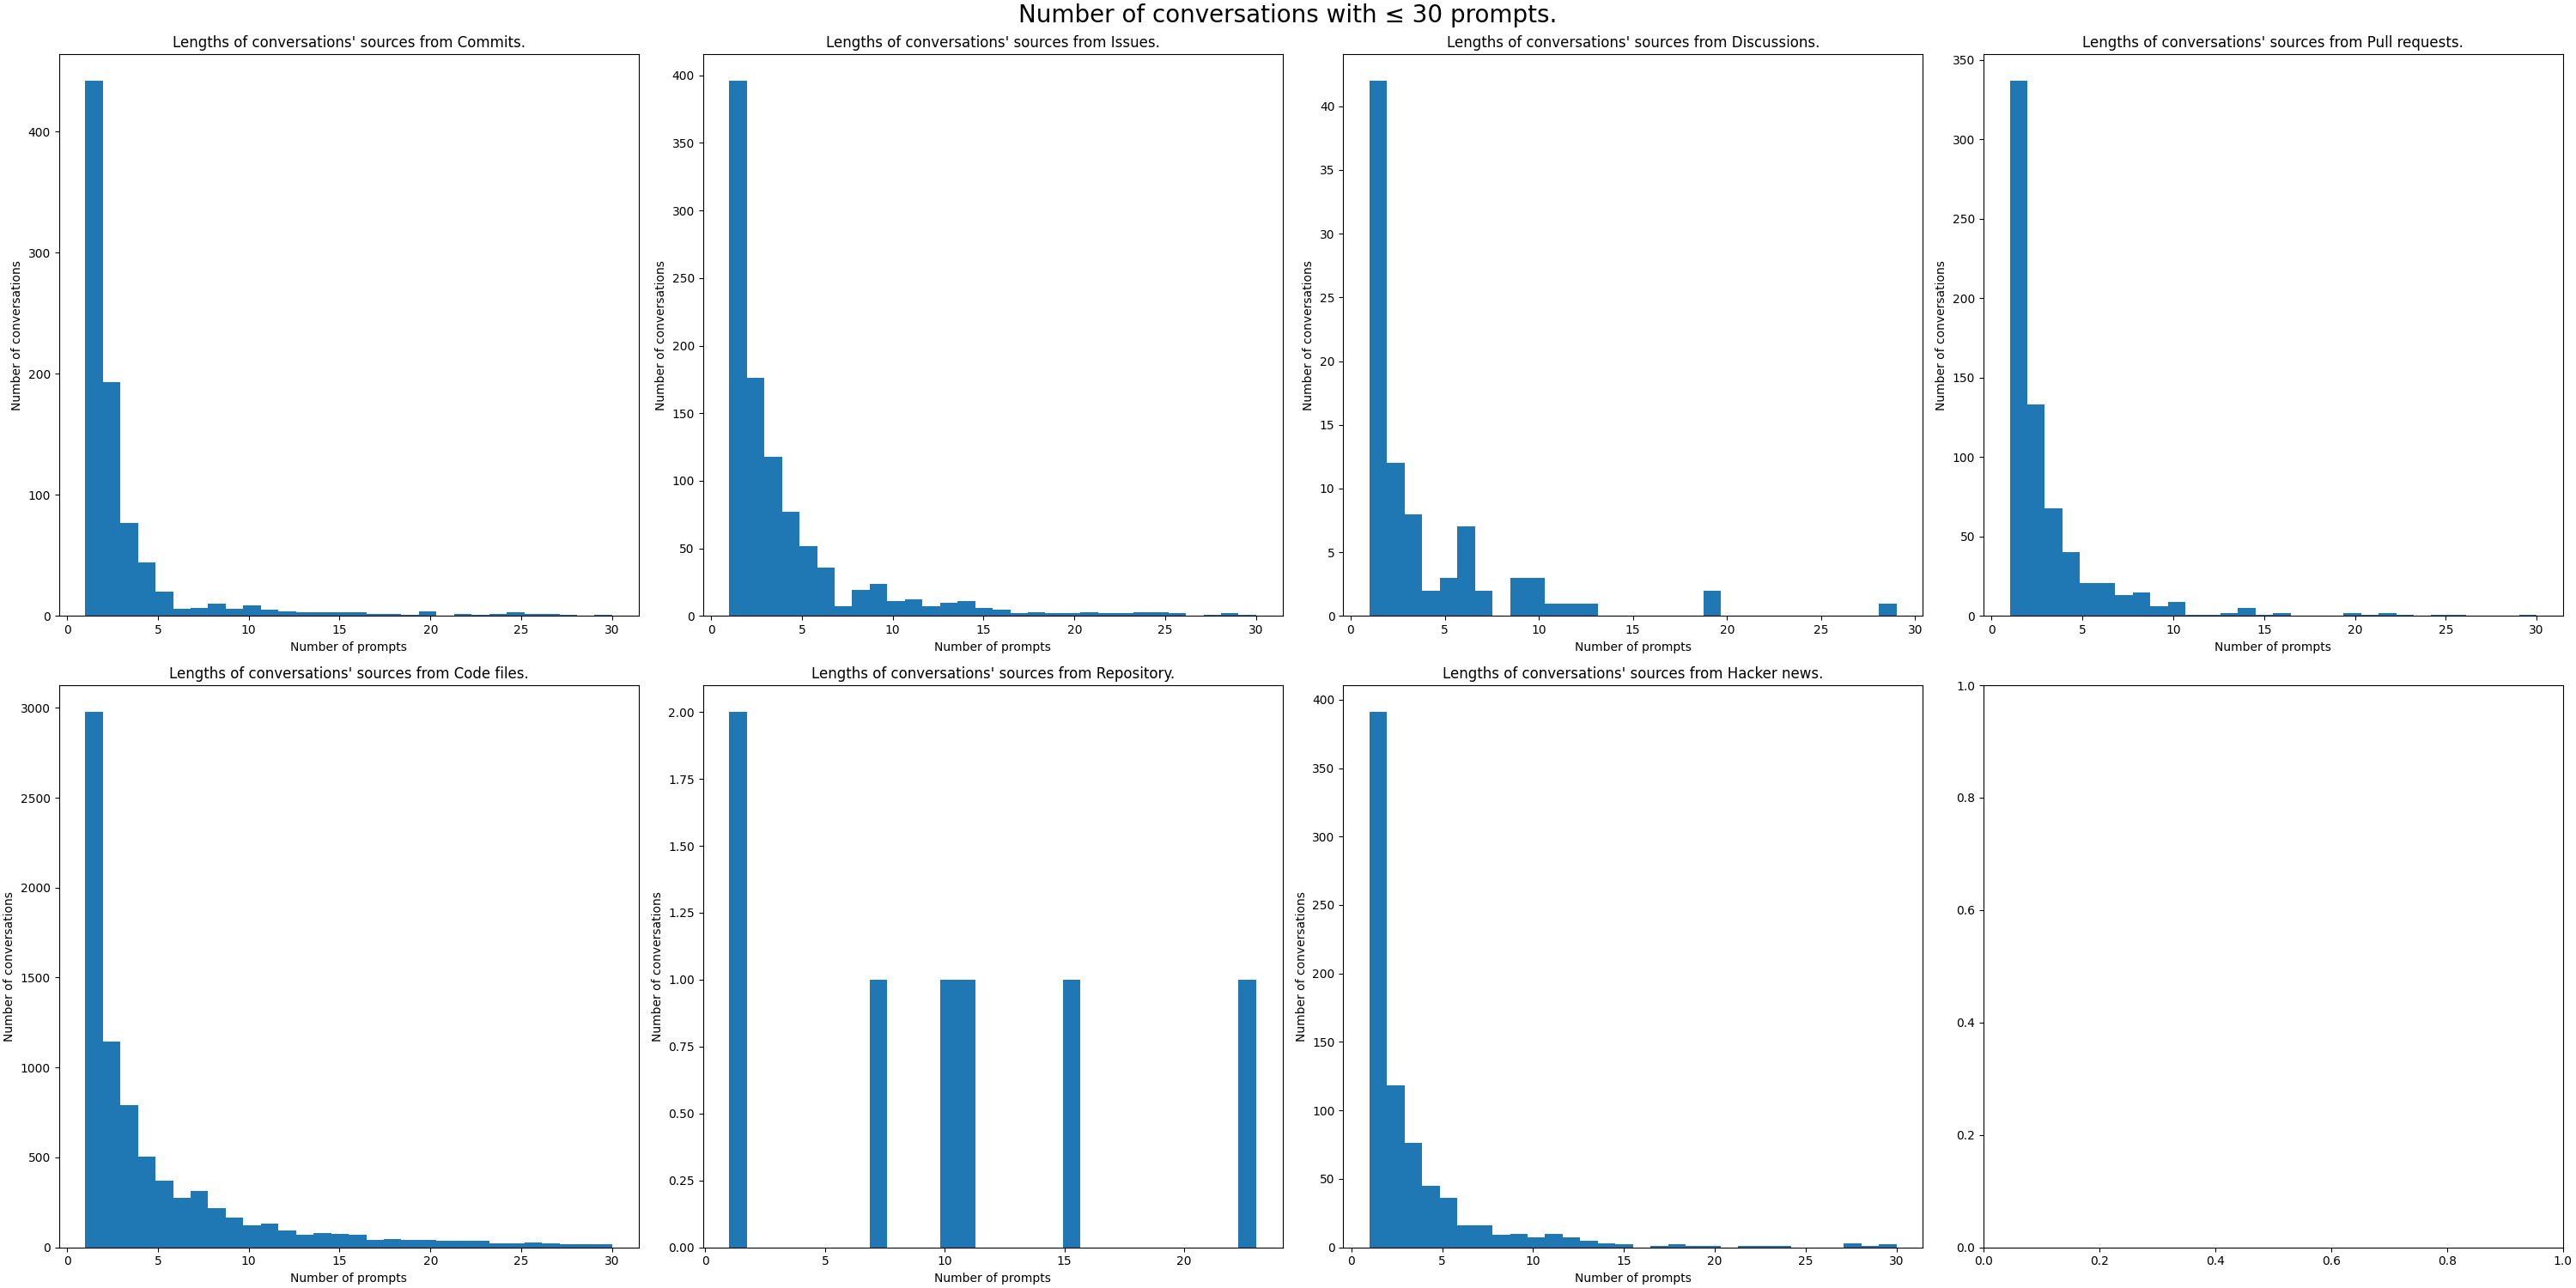
\includegraphics[width=\textwidth]{imgs/conv-per-prompt-nr.png}
    \caption{Number of conversations per prompt number for all conversation sources.}
    \label{fig:conv-per-prompt}
\end{figure}

\subsubsection{Outliers and their content}
The conversations that are too long are saved to the file and investigated manually for the reasons why they contain that many prompts. Doing that we managed to find the following reasons on why they were that long:
\begin{itemize}
    \item Conversation contains several prompts of text that did not fit into one prompt due to the set character limit: users were copying the whole code files, articles or books.
    \item Users were asking for code snippets, and the code provided from \gls{gpt} either did not correspond to user expectations and the request had to be modified several times by the user, or the code returned the errors, that users were not able to solve and had to ask for help from \gls{gpt}.
    \item Users used \gls{gpt} for programming: they provided with the information what they want it to program, asking \gls{gpt} to write the code, while testing it on their machine and providing with the feedback on the errors received or what needs to be changed.
    \item Users use \gls{gpt} as their mentor: they post the code they wrote asking for explanation or improvements suggestions. Occasionally posting errors it produced and asking for help or explanation.
    \item Users use \gls{gpt} for conversations that are not related to the programming issues: talking about \gls{gpt} opinions on different topics, asking for advice or asking more general questions; 
\end{itemize}

\subsubsection{Average symbol/word count per prompt}
The number of symbols and words per prompts varied significantly depending on the source of the conversation. However, the graphs for the number of symbols and the number of words per each source are comparable, where the peaks and troughs on the graphs are present at the same locations. Thus, we will look at both the number of symbols and the number of words together to investigate the outliers that have too high symbol/word count.

Figure~\ref{fig:symbols-per-prompt} and \ref{fig:words-per-prompt} show the average number of symbols and words per current prompt number, respectively. Axis \textit{x} represents the prompt number, where minimum value is 1 and maximum value is the number of prompts in the longest conversation of this dataset. Axis \textit{y} shows the average count of symbols/words that prompt \textit{x} has. One important factor that influences the way graphs look like is the length of conversations. The graphs show average count of symbols/words for the prompt number: some conversations are shorter than others, meaning that longer conversations have more influences on the average symbol/word count for the higher prompt counts, since the average is calculated on the lower number of prompts. A good example of it is GitHub discussion dataset, which has only one conversation longer than 19 prompts, meaning that the average symbol/word count for prompts 20 to 29 is taken from one conversation, which results in peaks on the graphs. GitHub code files dataset shows different behaviour: longest conversations have lower symbol/word counts. However, in all datasets first prompts are usually used to introduce the problem \gls{gpt} needs to solve, which requires a more thorough description of the problem; thus, resulting in a higher symbol/word count.

To investigate the outliers, we have selected the cut-off points for each dataset separately. The cut-off point is selected to be 2/3 of the maximum average. Conversations containing prompts longer than the cut-off points were saved for the further investigation. GitHub commits and HackerNews datasets have smooth graphs with little fluctuation, thus, they are not included in outlier investigation process. For all the other four datasets we have selected the following cut-off points:
\begin{itemize}
    \item GitHub issues: prompt length in symbols of 400 or more;
    \item GitHub discussions: prompt length in symbols of 800 or more;
    \item GitHub pull request: prompt length in symbols of 800 or more;
    \item GitHub code files: prompt length in symbols of 850 or more;
\end{itemize}

\begin{figure}[H]
    \centering
    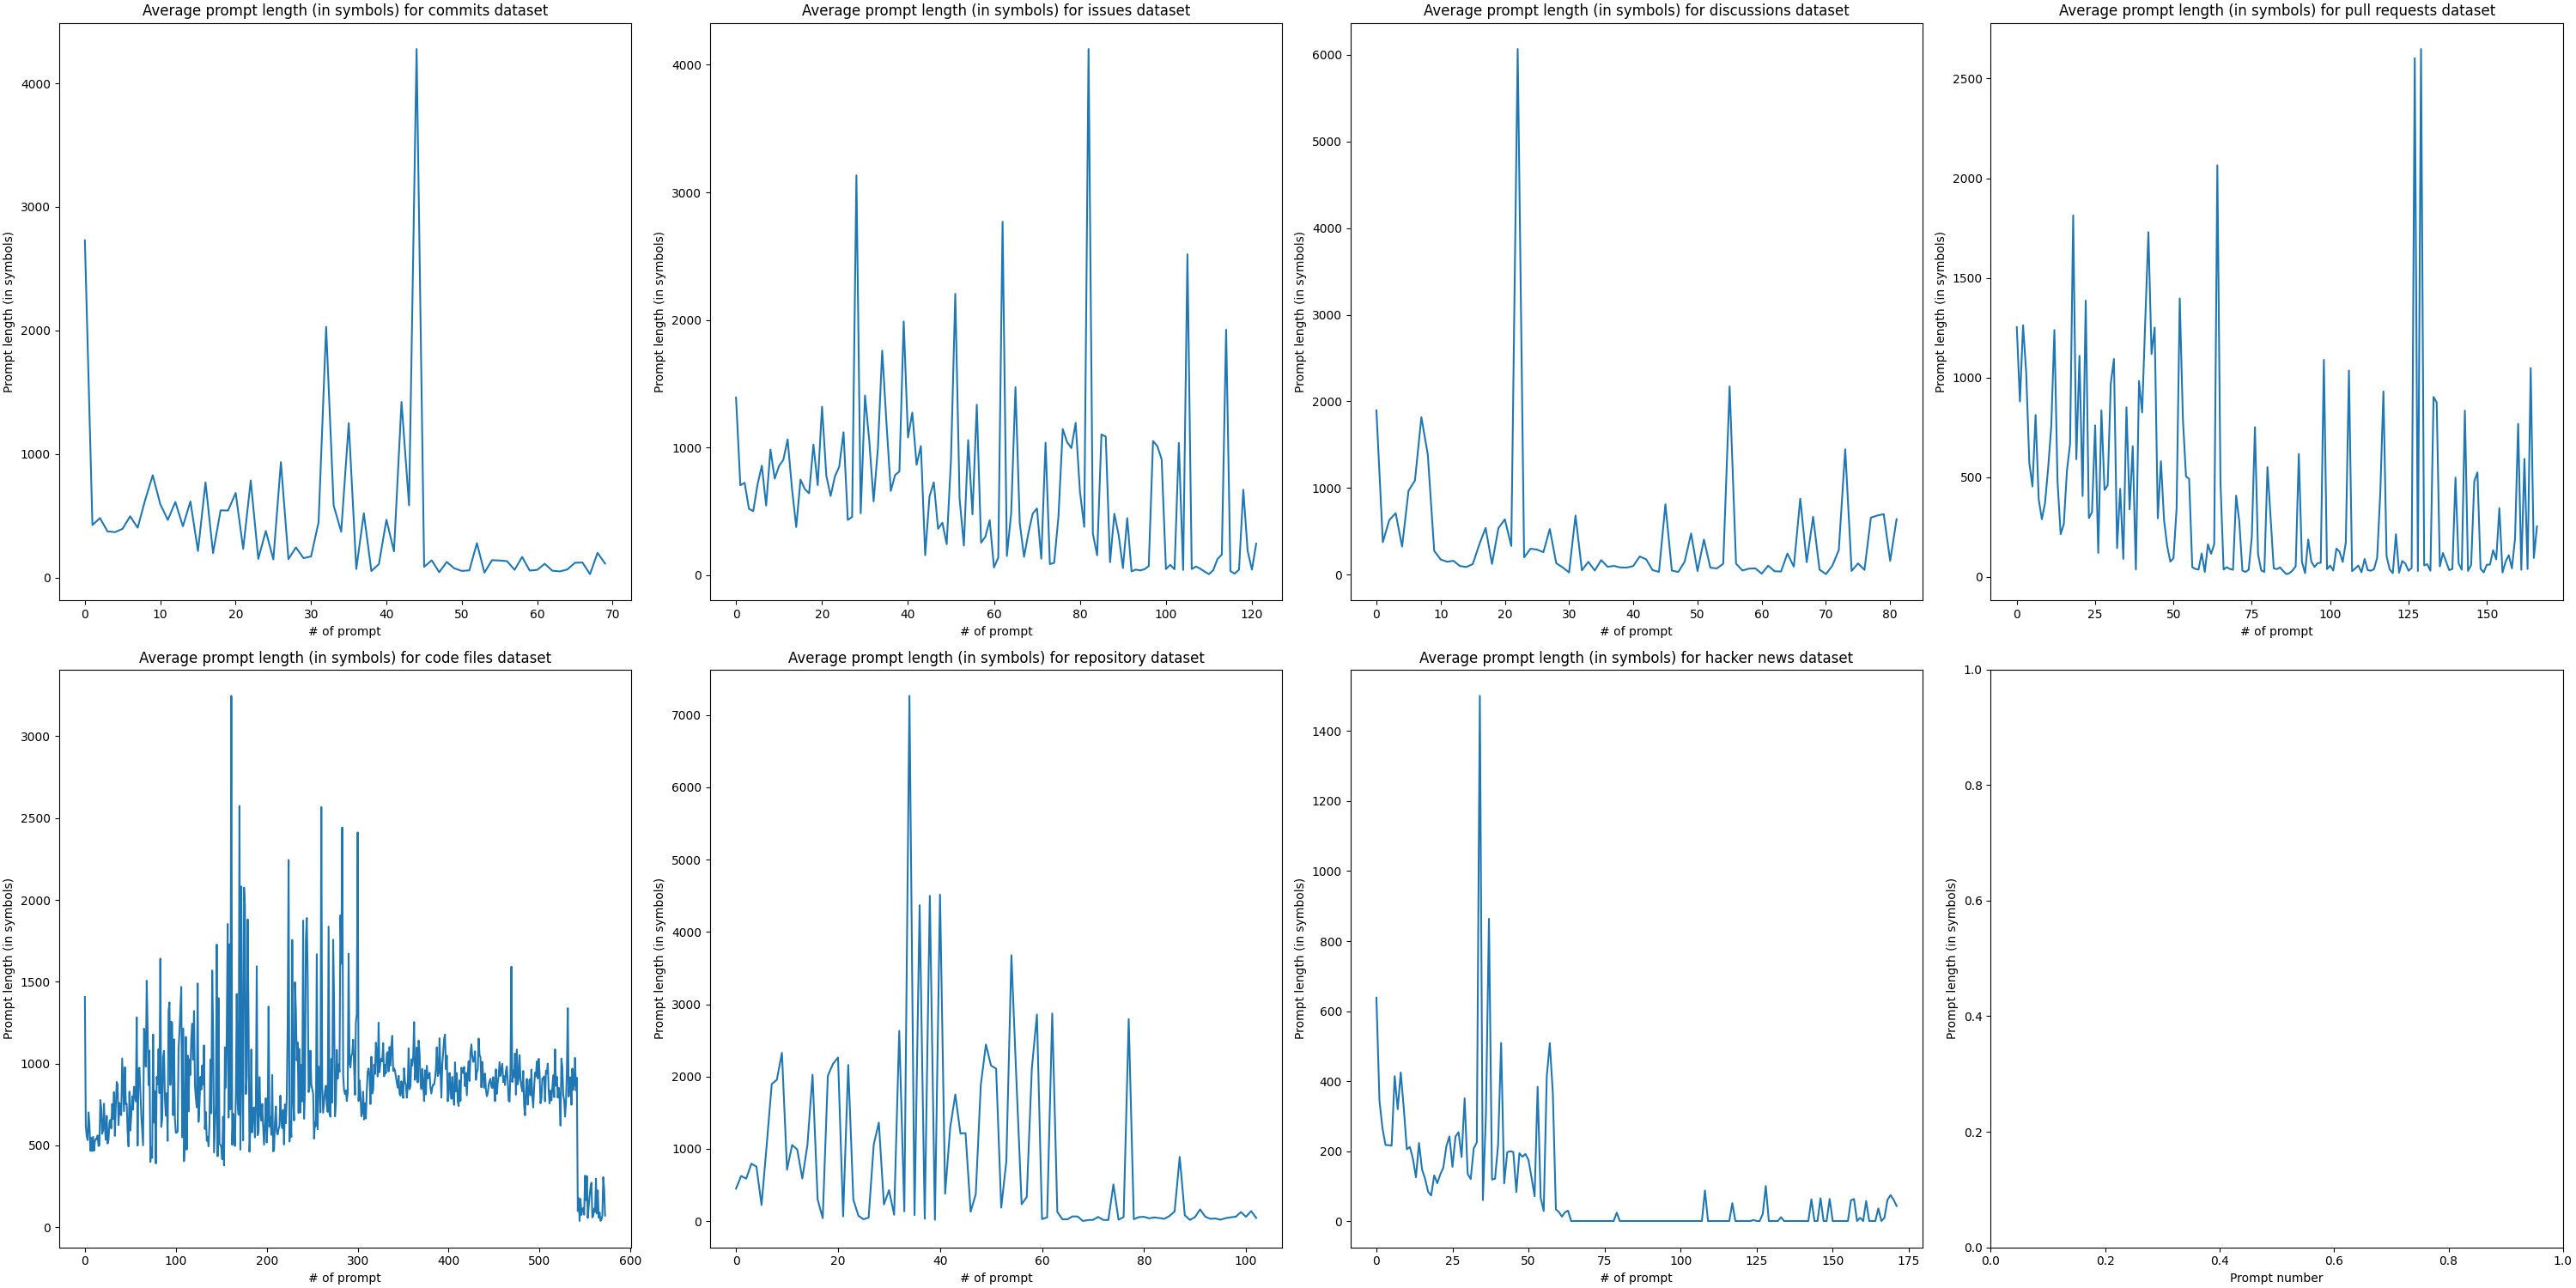
\includegraphics[width=\textwidth]{imgs/symbols-per-prompt.png}
    \caption{Average symbol count per prompt number for all conversation sources after code lines were removed.}
    \label{fig:symbols-per-prompt}
\end{figure}

\begin{figure}[H]
    \centering
    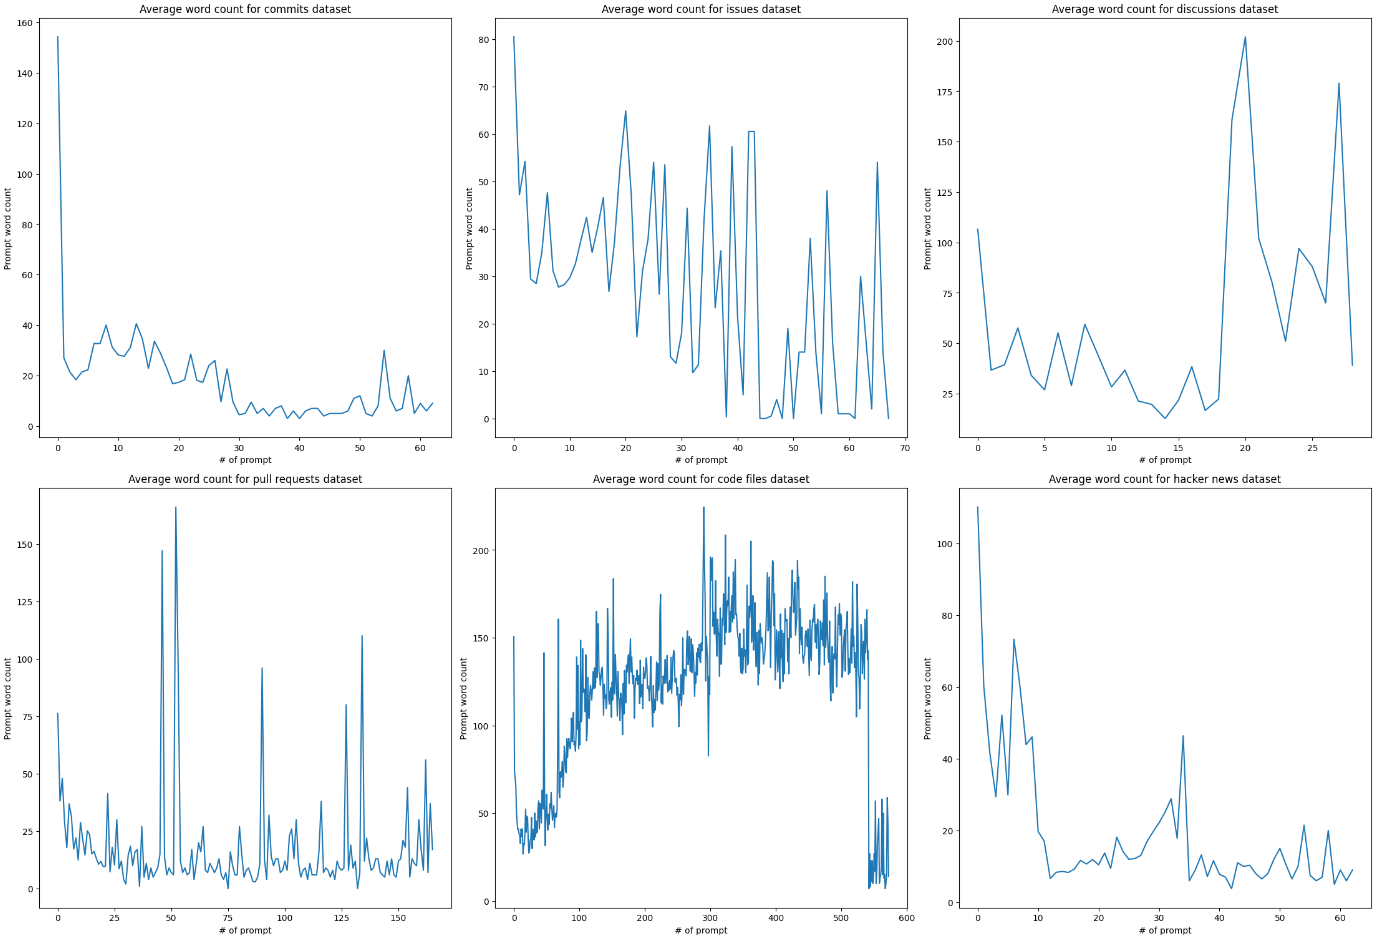
\includegraphics[width=\textwidth]{imgs/word-count-per-prompt.png}
    \caption{Average word count per prompt number for all conversation sources after code lines were removed.}
    \label{fig:words-per-prompt}
\end{figure}

\subsubsection{Outliers and their content}
The conversations containing very long prompts are saved to the file, and their content is investigated manually to identify the reasons that explain their length. We have managed to identify the following content categories in long prompts:
\begin{itemize}
    \item Prompt contains long text that was pasted by the user from the external source (scientific article, GitHub issue description, code documentation, etc.), and user wants to get the analysis or explanation of the text or its part, or wants to get the rewritten version to match the target audience.
    \item Prompt contains error message, code documentation/comments and code parts (that were not detected by program line detection function) that user wants to fix, debug, get feedback on.
    \item Prompt contains a thorough description of the problem the user is facing, which can contain:
    \begin{itemize}
        \item A very detailed problem description, when the user knows exactly what they want to receive from \gls{gpt};
        \item A problem description in a poetic way (usually asking \gls{gpt} to play a certain role: e.g. teacher, mentor, area expert);
        \item User provides relevant for the problem background information to \gls{gpt};
        \item Multiple questions regarding the problem or provided solution; 
        \item What solutions user found, which did not work;
        \item Long URL links;
        \item The list of requirements or instructions;
        \item Example of the output, functionality, or code user wants to receive.
    \end{itemize}
\end{itemize}

\section{Data preparation} \label{sec:data-prep}
In order to perform further analysis, we have pre-processed the remaining data using lemmatisation and tokenisation processes.  

During lemmatisation process we split sentences into a list of structures: words, punctuation, digits or alphanumeric values; and lemmatise them using \textit{lemmatize\_sentence} function from \textbf{pywsd} package~\cite{pywsd14}. The function tries to convert a surface word into lemma, and if lemmatize word is not in wordnet then try and convert surface word into its stem. 

Once all the sentences are lemmatised, they are cleaned from the non-relevant data. We remove the following tokens: 
\begin{itemize}
    \item Links: token starts with \textit{"http"};
    \item Stop words: the selection of \textit{stop\_words} from \textbf{nltk} package\footnote{\href{https://www.geeksforgeeks.org/removing-stop-words-nltk-python/}{Stop words list}}~\cite{nltk};
    \item Punctuation; 
    \item Word contains digits.
\end{itemize}

Lemmatised and cleaned lists of tokens are then further passed on to the functions that conduct further analysis on the content of the cleaned sentences. 

\section{N-grams}
N-grams is a sequence of \textit{n} consecutive characters, words or other textual structures~\cite{n-grams}, where \textit{n} is the number of such structures in a pair. The set of n-grams is obtained by shifting the box of \textbf{n} structures through the data and retrieving the values. The structures order is kept when the n-grams are being extracted. In this research we focus on the words, so the sentence \textit{"That fox is chasing a rabbit"} can be split into the following structures: ${that, fox, is, chasing, a rabbit}$. We can create the following n-grams from the mentioned set of words:
\begin{itemize}
    \item Bi-grams: $(that, fox)$, $(fox, is)$, $(is, chasing)$, $(chasing, a)$, $(a, rabbit)$; 
    \item Tri-grams: $(that, fox, is)$, $(fox, is, chasing)$, $(is, chasing, a)$, \\$(chasing, a, rabbit)$;
    \item Quadri-grams: $(that, fox, is, chasing)$, $(fox, is, chasing, a)$, \\$(is, chasing, a, rabbit)$;
\end{itemize}

Before the data is used for n-grams extraction, the data is cleaned from stop words, as described in Section~\ref{sec:data-prep}. In the example above it would mean that words \textit{"that"}, \textit{"is"} and \textit{"a"} will be removed in the pre-processing step. All the other context carrying words are used to create n-grams for the data. N-grams are created using \textit{ngrams()} function from \textbf{nltk} package, where \textit{n} is set to the desirable value. The extracted n-grams are used to create n-grams frequency distribution: all the same n-grams are grouped together and their frequency is calculated. Such frequency distribution allows us to order all the extracted n-grams in descending order based on their frequency and focus our analysis on the most frequent n-grams. 

For easier visualisation, we use WordCloud package~\cite{wordcloud} that generates word clouds where the most common n-grams use bigger font size, while less common ones use smaller font sizes that is dependent on their frequency.

\section{Topic modelling}
Topic models are generative models that provide a probabilistic framework~\cite{topic-model}. These models are used for large electronic text collections to organise, understand, search and summarise their content. 

The topics are the relations that link words in a vocabulary and their occurrence in documents. Each document is viewed as a mixture of topics. Topic models discover different themes present in the text collections and annotate the documents according to the themes. The document coverage distribution of topics is then generated to provide an overview of topics found in this document collection. 

In this study we use \gls{lda} topic modelling -- one of the most popular text modelling techniques. \gls{lda} is a probabilistic generative model that allows the observations to be described by unobserved data that explains why some parts of the data are similar to each other~\cite{tong-topic-modelling}. In \gls{lda}, documents consist of multiple topics and each topic is a distribution over a fixed vocabulary. For example, if we have the  following vocabulary of \{\textit{pan, cook, football, basketball}\}, then the kitchen topic will assigne high probabilities to the words \textit{pan} and \textit{cook}, while \textit{football} and \textit{basketball} will have very low probabilities; however, the sport topic will have the opposite probabilities for all the words. 

In the implementation we use the data cleaned in the pre-processing step as described in Section~\ref{sec:data-prep}. We start with creating the vacabulary: this is done using \textit{CountVectorizer} class to convert a collection of text documents to a matrix of token counts~\cite{scikitlearnCountVectorizer}. The parameters of \textit{min\_df} and \textbf{max\_df} are set to 0 and 1 respectively; \textit{ngram\_range} is set to tuple of (1,4), making vocabulary to consist of n-grams of the length 1 to 4 words; and the stop words are the stop words from \textbf{nltk} package. For topic modelling we use \textit{LatentDirichletAllocation} class from \textbf{sklearn} package~\cite{scikitlearnLatentDirichletAllocation}\todo{Code: remove split, use fit\_transform}, where we set number of topics to 10, iteration count to 6 and random state to 42. We calculate perplexity and coherence score of the topic model and visualise them along with WordCloud visualisation of the topics. 

\section{Sequence mining}
\todo{add}

\section{Limitations}
There exist limitations of the dataset and methods selected for this study that influence the results of the research. These limitation are addressed in this section. 

Dataset used for this study provides a good overview of how developers use \gls{gpt} for solving their daily problems. However, the sources that were used to extract this knowledge are not completer. The conversation data was collected from GitHub (commits, code files, discussions, pull requests and issues) and HackerNews, and it covers the conversations that happened between the release date of \gls{gpt} and 12th of October 2023. Thus, the data is not complete and misses other sources that could contain more knowledge regarding the use of \gls{gpt} by developers. Additionally, since the data was last sourced over a year ago, the conversations that happened after the mentioned date and conversations with \gls{gpt} that uses newer version GPT-4\footnote{\url{https://openai.com/index/gpt-4/}} are not included in this dataset. Moreover, some conversation links that were used to scrape the data are not working anymore, thus, the validity of these conversations cannot be checked.

Additionally, the language detection tool and the data cleaning method used are not fully accurate and miss prompts or prompt lines that contain foreign language and code. It was discovered, that the prompts often contain pasted text (articles, documentation, code comments) and error messages, which are hard to detect using the selected tool set, since they contain sentences in natural English language, but do not contain the information needed for answering the research question. Thus, the code snippets, foreign language prompts and copied texts add noise to the data that the tools are not able to detect.
\chapter{Results}\label{results}
In this chapter we provide insights into the knowledge we managed to extract during the analysis of developers prompts in developer-\acrshort{gpt} interaction. This chapter focuses on the results extracted from N-grams, topic modelling and sequence mining of the prompts. 

\section{N-grams}
N-grams are extracted in order to provide an overview of the most common lexical patterns found within the data. Data gathered from each source was analysed separately and the most common 1- to 4-grams were extracted. Table~\ref{table:common-ngrams} shows interesting tri- and quadri-grams extracted from various data sources. 

\begin{longtable}{|l|c|m{8cm}|}
    \hline
    Source & n & Found n-grams  \\
    \hline
        \multirow{2}{*}{GitHub commits} & 3 & shell script create, encode enclose result, avoid use sed, implement following feature  \\
        \cline{2-3}
        & 4 & script create change file, avoid use sed favor, task implement following feature \\
    \hline
        \multirow{2}{*}{GitHub issues} & 3 & th block th, valid string generation, state lookahead token, kernel patch instal \\
        \cline{2-3}
        & 4 & td th block th, string generation metadata information, metadata information visit input, community edition line module \\
    \hline
        \multirow{2}{*}{GitHub discussions} & 3 & technology feasibility stable, operational feasibility challenge, clause potentially unfair, employee desirability mixed/high, open/close code environment \\
        \cline{2-3}
        & 4 & technology feasibility stable employee, employee desirability high team \\
    \hline
        \multirow{2}{*}{GitHub pull requests} & 3 & gazebo sensor imu, plugin sensor accelerometer, deprecate pip enforce, possible replacement use  \\
        \cline{2-3}
        & 4 & coelemic cavity lumen subclassof, gazebo sensor imu plugin, sensor accelerometer parent origin, replacement use pip package, string sure want delete \\
    \hline
        \multirow{2}{*}{GitHub code files} & 3 & rdf type owl, restriction owl minqualifiedcardinality, passage book rewrite, break fourth wall\\
        \cline{2-3}
        & 4 & rdf type owl objectproperty, rdfs subpropertyof owl topobjectproperty, george r r martin, book rewrite passage remove, break fourth wall include, wall include reference reader \\
    \hline
        \multirow{2}{*}{GitHub repositories} & 3 & fill height viewport, increase understanding universe, help reduce suffering, research educational institution \\
        \cline{2-3}
        & 4 & height fill height viewport, leave position foreground scyscraper, reduce suffering increase prosperity, prosperity increase understanding universe, planet intellectual community train \\
    \hline
        \multirow{2}{*}{Hacker News} & 3 & capture position position, form line capture, tic tac toe, session user host, level level headline \\
        \cline{2-3}
        & 4 & form line capture position, x currently form line, headline insert concat star, concat star schedule progn \\
    \hline
\caption{Interesting 3- and 4-grams extracted from the data.}
\label{table:common-ngrams}
\end{longtable}

The extracted n-grams reveal distinct linguistic and thematic patterns across different data sources. Prompts from GitHub commits and pull requests use task-oriented, direct and action-driven communication typical of development workflows. The prompts often focus on modifying, automating or improving code artefacts. In contrast, GitHub discussions contain  planning-related n-grams like ``clause potentially unfair'' and ``technology feasibility stable employee'', suggesting that contributors debate feasibility and desirability of the solution, not just technical correctness. 

GitHub repositories show recurring themes in UI rendering (e.g.m CSS and Viewport references) as well as humanitarian, educational, and scientific discussions. However, prompts from GitHub issues and code files is influenced by embedded code or markup, such as HTML and RDF/OWL artefacts --- indicating developers often seek help with specific technical problems.

Hacker News conversations differ by a less technical, more playful approach. N-grams like ``tic tac toe'', ``form line capture position'', and ``headline insert concat star'' combine elements of game logic, syntax play, and UI behavior, typical of exploratory or playful community posts.

In conclusion, each platform reflects its users’ intent --- ranging from practical coding to ethical reflection to creative exploration.

\section{Topic modelling}

\section{Sequence mining}
\chapter{Discussion and conclusion}\label{conclusions}


\bibliographystyle{ieeetr}
\bibliography{bibliography}

\printglossary

\chapter*{Reflection on research process} \label{reflection}

\begin{itemize}
    \item Reflection on the research results
    \item Reflection on the process
    \item Problems encountered
    \item Takeaways 
\end{itemize}

\appendix
\chapter{Appendix}\label{appendix}


\end{document}
